% ============================================================
% Application: Perturb-seq (Norman et al., 2019)
% ============================================================

\begin{frame}{Application: Perturb-seq (Norman et al., 2019)}
  \vspace{1ex}
  \row{Data}{$\cD$: 8,907 control cells; \; 99,590 perturbed cells}
  \row{Interventions}{CRISPR activation of 1 or 2 of 105 genes $\to$ $K = 217$ datasets (50--2,000 cells each)}
  \row{Observed $X$}{expression of 5,000 highly variable genes}
  \row{Model}{$p = 105$ latents (one per target gene), \; shift interventions}
  \sep
  \row{Train}{$\cD$ + 105 single-gene datasets \; (96 cells held out for each of the 14 largest)}
  \row{Test}{held-out single-gene cells + all 112 double-gene perturbations (\textbf{never seen})}
  \par\centering
  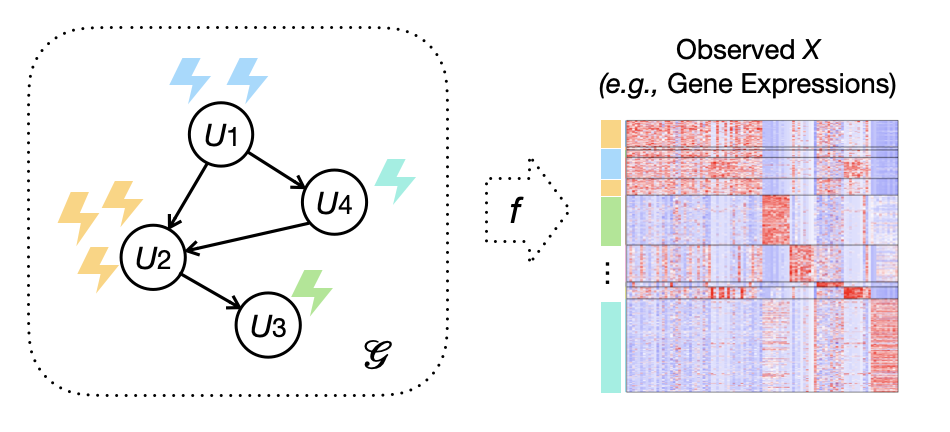
\includegraphics[width=0.36\textwidth]{perturbseq_overview}

  \note{
    ~1.5 min
    \begin{itemize}
      \item Perturb-seq: CRISPR perturbation + single-cell RNA-seq. CRISPRa increases expression of the target gene; its regulators still act on it, so it is a soft intervention. Modelled as a shift intervention, exactly the $a^I$ from the VAE.
      \item Data after preprocessing: 8,907 control cells (observational $\cD$) and 99,590 perturbed cells; targets: 1 or 2 out of 105 genes, $K = 217$ interventional datasets (105 single + 112 double), 50 to 2,000 cells each.
      \item Each cell = vector of 5,000 highly variable genes ($X$).
      \item Latent dimension $p = 105$ = number of targeted genes.
      \item Training: all control cells + the 105 single-gene datasets. For each single-gene dataset with more than 800 cells (14 of them), 96 cells are held out for testing.
      \item All 112 double-gene perturbations are held out completely: a test of extrapolation to unseen combinations.
    \end{itemize}
  }
\end{frame}

% ------------------------------------------------------------
\begin{frame}{Results: predicting perturbation effects}
  \vspace{1ex}
  \centering
  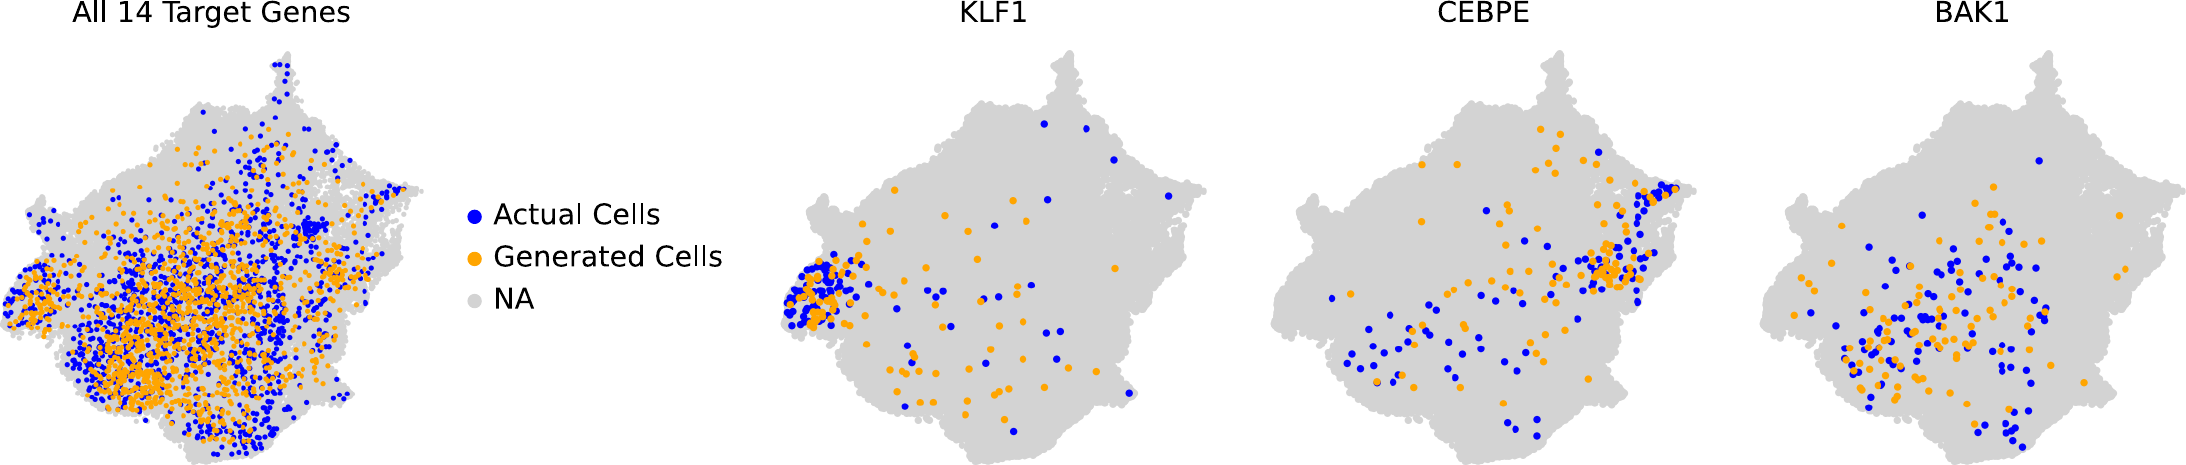
\includegraphics[width=0.88\textwidth]{results_umap}
  \par\smallskip
  {\small UMAP: \textbf{actual} held-out cells (blue) \; vs.\ \; \textbf{generated} cells (orange)}
  \par\medskip\raggedright
  \row[3.6cm]{Single gene (seen)}{$R^2 \approx 0.99$ all genes, \; 0.95 top-20 DE genes}
  \row[3.6cm]{Double gene (unseen)}{$R^2 \approx 0.98$ all genes, \; 0.88 top-20 DE genes}
  \row[3.6cm]{Failures}{some pairs $\to$ wrong subpopulation \; (non-additive gene interactions?)}

  \note{
    ~1.5 min
    \begin{itemize}
      \item UMAP of all cells (grey); blue = actual held-out cells, orange = generated virtual counterfactuals for the same intervention. The generated cells land in the right subpopulations (e.g.\ KLF1: a small cluster at the left).
      \item $R^2$ is computed by regressing the mean of the generated samples on the mean of the true interventional distribution (App.\ G); ``DE genes'' = the 20 most differentially expressed genes for that intervention, the harder test.
      \item Single-gene interventions (seen in training, evaluated on held-out cells): $R^2 \approx 0.99$ on all genes, 0.95 on top-20 DE genes.
      \item Double-gene interventions were never seen: the model predicts them by adding the two learned shifts in the latent space (the extrapolation from Theorem 3). $R^2 \approx 0.98 / 0.88$.
      \item Some pairs land in the wrong subpopulation; the authors suggest these gene pairs may act non-additively, which a sum of shifts cannot capture.
    \end{itemize}
  }
\end{frame}

% ------------------------------------------------------------
\begin{frame}{Results: learned gene-program DAG}
  \vspace{1ex}
  \begin{itemize}
    \item Shrink $p$ until targets cover all latents $\to$ \; $p = 7$ gene programs
    \item Several runs, keep the \textbf{sparsest} DAG
    \item Recovers \textbf{DUSP9} $\to$ \textbf{MAPK1}, \textbf{DUSP9} $\to$ \textbf{ETS2} \; (validated by Norman et al.)
    \item MAPK1 / ETS2: overlapping clusters $\to$ \; same latent node
  \end{itemize}
  \par\medskip\centering
  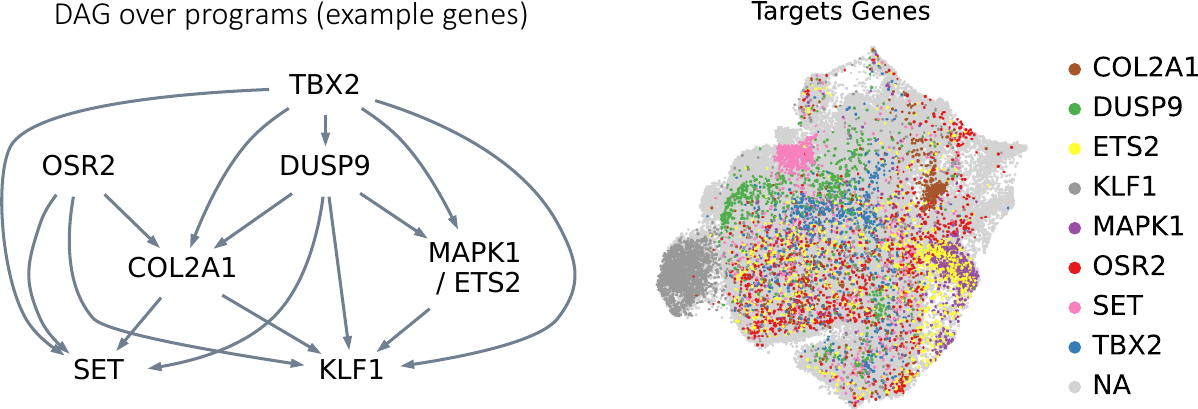
\includegraphics[width=0.6\textwidth]{learned_dag}

  \note{
    ~1 min
    \begin{itemize}
      \item To get an interpretable graph, $p$ is reduced from 105 until the learned targets of the 105 single-gene interventions cover all latent nodes: $p = 7$. Genes sharing a latent node form a ``program''.
      \item With $p = 7$ fixed, the algorithm is run several times and the DAG with the fewest edges is kept (the sparsity principle from the theory).
      \item Left: learned DAG over programs, labelled with example genes. It recovers DUSP9 $\to$ MAPK1 and DUSP9 $\to$ ETS2, which Norman et al.\ validated (their Fig.~5).
      \item MAPK1 and ETS2 share one node: their perturbation clusters overlap heavily (right, UMAP), so the model cannot separate them.
    \end{itemize}
  }
\end{frame}
